\documentclass[10pt,a4paper]{article}
\usepackage[a4paper,margin=21mm,top=20mm,bottom=22mm]{geometry}

\usepackage{amsmath,amssymb,mathtools,braket,bm}
\usepackage{graphicx,booktabs,array,tabularx,enumitem,caption,xcolor}
\usepackage{tikz}
\usetikzlibrary{arrows.meta,positioning}
\usepackage[expansion=false]{microtype}
\usepackage{fancyhdr}
\usepackage[colorlinks=true,linkcolor=blue!50!black,citecolor=blue!50!black,urlcolor=blue!50!black]{hyperref}

\definecolor{qblue}{HTML}{2A78D6}
\definecolor{qgrey}{HTML}{52514E}
\captionsetup{font=small,labelfont=bf}
\setlist{itemsep=1pt,topsep=3pt}
\setlength{\parskip}{3pt}
\setlength{\emergencystretch}{3em}
\pagestyle{fancy}\fancyhf{}
\renewcommand{\headrulewidth}{0pt}
\fancyfoot[L]{\footnotesize\color{qgrey}Quantivex v1.2.1 --- Physics of the backend}
\fancyfoot[R]{\footnotesize\color{qgrey}\thepage}

\newcommand{\Ha}{\,\mathrm{Ha}}
\newcommand{\mHa}{\,\mathrm{mHa}}
\newcommand{\Ang}{\ensuremath{\,\text{\normalfont\AA}}}
\newcommand{\cre}[1]{a^{\dagger}_{#1}}
\newcommand{\ann}[1]{a_{#1}}
\newcommand{\code}[1]{\texttt{\small #1}}

\title{\vspace{-8mm}\textbf{The physics inside Quantivex}\\[3pt]
\large From a calibration file and a molecule to a trust verdict:\\ every model, equation and approximation used by the backend}
\author{Technical companion to Quantivex v1.2.1}
\date{October 2026}

\begin{document}
\maketitle
\thispagestyle{fancy}

\begin{abstract}
\noindent Quantivex answers questions such as ``Which qubits of \texttt{ibm\_torino} should I use for N$_2$ at $2.0\Ang$, and can I trust the result?''. An LLM chooses which analyses to run, but every number is computed by deterministic code. This document states, precisely, the physics and mathematics behind that code. It covers: the electronic-structure problem and its active-space reduction; the Jordan--Wigner mapping to qubits; the unitary coupled-cluster variational eigensolver; the hardware noise model built from calibration data; qubit-chain selection by estimated success probability; shot-based energy estimation with readout-error mitigation; the statistics behind the verdict; how the plain-English answer is kept consistent with the computed numbers; and the Quantum Blur image transform. Each step names the corresponding source module, the approximation it makes, how it was validated, and the literature it rests on. Numbers quoted are those produced by v1.2.1 on the bundled \texttt{ibm\_torino} calibration snapshot (2025-02-26).
\end{abstract}

\tableofcontents

%=====================================================================
\section{Overview of the pipeline}
%=====================================================================
\begin{figure}[h]
\centering
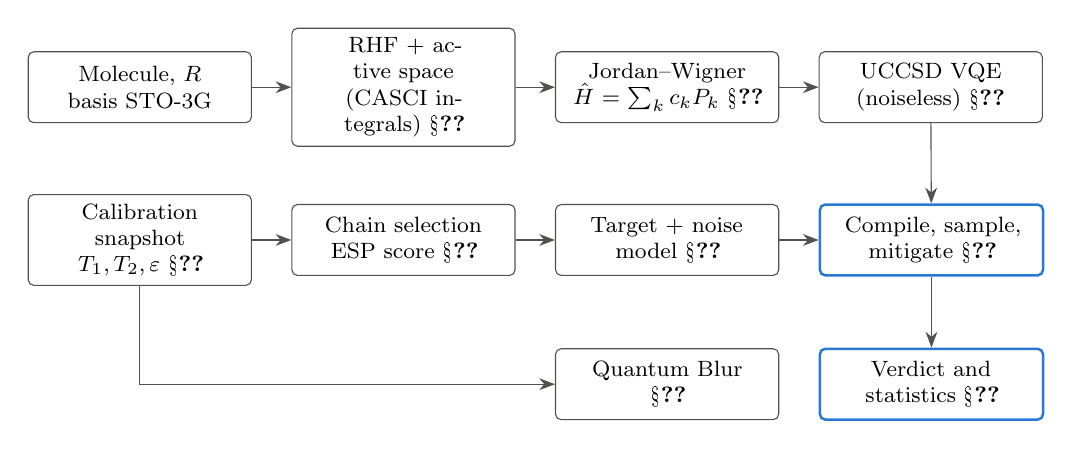
\begin{tikzpicture}[node distance=4mm and 5mm, every node/.style={font=\footnotesize},
 box/.style={draw=qgrey,rounded corners=2pt,align=center,minimum height=9mm,text width=26mm,fill=white},
 hl/.style={box,draw=qblue,line width=0.9pt},
 arr/.style={-{Stealth[length=2mm]},qgrey}]
\node[box] (mol) {Molecule, $R$\\ basis STO-3G};
\node[box,right=of mol] (hf) {RHF + active space\\ (CASCI integrals) \S\ref{sec:es}};
\node[box,right=of hf] (jw) {Jordan--Wigner\\ $\hat H=\sum_k c_k P_k$ \S\ref{sec:jw}};
\node[box,right=of jw] (vqe) {UCCSD VQE\\ (noiseless) \S\ref{sec:vqe}};
\node[box,below=9mm of mol] (cal) {Calibration snapshot\\ $T_1,T_2,\varepsilon$ \S\ref{sec:hw}};
\node[box,right=of cal] (chain) {Chain selection\\ ESP score \S\ref{sec:chain}};
\node[box,right=of chain] (noise) {Target + noise\\ model \S\ref{sec:noise}};
\node[hl,right=of noise] (est) {Compile, sample,\\ mitigate \S\ref{sec:meas}};
\node[hl,below=9mm of est] (ver) {Verdict and\\ statistics \S\ref{sec:stats}};
\node[box,left=of ver] (blur) {Quantum Blur\\ \S\ref{sec:blur}};
\draw[arr] (mol)--(hf); \draw[arr] (hf)--(jw); \draw[arr] (jw)--(vqe);
\draw[arr] (cal)--(chain); \draw[arr] (chain)--(noise); \draw[arr] (noise)--(est);
\draw[arr] (vqe)--(est); \draw[arr] (est)--(ver); \draw[arr] (cal.south) |- (blur.west);
\end{tikzpicture}
\caption{Data flow. The top row is quantum chemistry and is independent of hardware. The middle row turns one calibration snapshot into a qubit choice and a noise model. The two meet when the optimised state is compiled onto chosen physical qubits and sampled under that noise.}
\label{fig:pipeline}
\end{figure}

\paragraph{Design principle.} The variational parameters are optimised \emph{noiselessly} (exactly), and the optimised state is then executed under the device noise model on a chosen layout. The resulting energy error therefore isolates the effect of hardware noise and qubit choice from optimiser noise. This is a deliberate, documented choice (\S\ref{sec:limits}).

\paragraph{Units and conventions.} Energies are in hartree ($1\Ha = 627.5095$~kcal/mol); errors are quoted in millihartree (mHa). Bond lengths are in \Ang. ``Chemical accuracy'' is $1$~kcal/mol $=1.5936\mHa$, rounded to $1.6\mHa$ in the code (\code{CHEMICAL\_ACCURACY\_HA}). Qiskit's little-endian convention is used throughout: in a basis state $\ket{b_{n-1}\cdots b_1 b_0}$, qubit $j$ is bit $b_j$, and the basis index is $\sum_j b_j 2^j$.

%=====================================================================
\section{The electronic-structure problem}\label{sec:es}
%=====================================================================
\subsection{Molecular Hamiltonian}
Within the Born--Oppenheimer approximation~\cite{BornOppenheimer1927}, nuclei are fixed at separation $R$. The electronic Hamiltonian, in atomic units, is
\begin{equation}
\hat H_{\mathrm{el}} = -\sum_i \tfrac12\nabla_i^2 - \sum_{i,A}\frac{Z_A}{|\mathbf r_i-\mathbf R_A|} + \sum_{i<j}\frac{1}{|\mathbf r_i-\mathbf r_j|} + E_{\mathrm{nn}},\qquad E_{\mathrm{nn}}=\frac{Z_1Z_2}{R}.
\end{equation}
Quantivex supports N$_2$, H$_2$ and LiH, all placed along the $z$ axis, in the minimal STO-3G basis~\cite{Hehre1969}. Each basis function is a fixed contraction of three Gaussians fitted to a Slater orbital.

\subsection{Restricted Hartree--Fock}
The closed-shell (RHF) mean-field solution solves the Roothaan--Hall equations~\cite{Roothaan1951,SzaboOstlund}
\begin{equation}
\mathbf F(\mathbf C)\,\mathbf C=\mathbf S\,\mathbf C\,\bm\varepsilon ,
\end{equation}
self-consistently, where $\mathbf F$ is the Fock matrix, $\mathbf S$ the overlap matrix, $\mathbf C$ the molecular-orbital (MO) coefficients and $\bm\varepsilon$ the orbital energies. The single determinant $\ket{\Phi_{\mathrm{HF}}}$ built from the lowest occupied MOs gives $E_{\mathrm{HF}}$. The \emph{correlation energy} is
\begin{equation}
E_{\mathrm{corr}} = E_{\mathrm{exact}} - E_{\mathrm{HF}} \le 0 ,
\end{equation}
which is the part a quantum computer is meant to recover. In the code: PySCF~\cite{PySCF2020} RHF with \code{conv\_tol}$=10^{-11}$, molecular point-group symmetry on, and a fixed occupation per irreducible representation (\S\ref{sec:irreps}).

\subsection{Active space and CASCI}
Only $n$ spatial orbitals (the \emph{active} space) are treated explicitly. Lower doubly occupied orbitals form an inactive \emph{core}, and the remaining virtual orbitals are discarded. With core orbitals $i,j$ and active orbitals $p,q,r,s$, the core is folded into an effective one-electron operator and a constant~\cite{Helgaker2000}:
\begin{align}
h^{\mathrm{eff}}_{pq} &= h_{pq} + \sum_{i\in\mathrm{core}} \bigl[\,2(pq|ii)-(pi|iq)\,\bigr],\\
E_{\mathrm{core}} &= E_{\mathrm{nn}} + \sum_{i\in\mathrm{core}}\Bigl[2h_{ii}+\sum_{j\in\mathrm{core}}\bigl(2(ii|jj)-(ij|ji)\bigr)\Bigr],
\end{align}
with two-electron integrals in chemists' notation
\begin{equation}
(pq|rs)=\iint \phi_p^*(\mathbf r_1)\phi_q(\mathbf r_1)\,\frac{1}{r_{12}}\,\phi_r^*(\mathbf r_2)\phi_s(\mathbf r_2)\,d\mathbf r_1 d\mathbf r_2 .
\end{equation}
The active-space Hamiltonian, in second quantisation with spin $\sigma,\tau\in\{\alpha,\beta\}$, is
\begin{equation}\label{eq:H2q}
\hat H = E_{\mathrm{core}} + \sum_{pq,\sigma} h^{\mathrm{eff}}_{pq}\,\cre{p\sigma}\ann{q\sigma} + \frac12\sum_{pqrs}\sum_{\sigma\tau}(pq|rs)\,\cre{p\sigma}\cre{r\tau}\ann{s\tau}\ann{q\sigma}.
\end{equation}
Exact diagonalisation of \eqref{eq:H2q} within the right particle number and spin gives the complete-active-space configuration-interaction (CASCI) energy. This is the reference ``exact'' energy $E_{\mathrm{exact}}$ in every Quantivex result. It is exact \emph{within the active space and basis}, not the experimental energy of the molecule. In the code, \code{mcscf.CASCI}, \code{get\_h1eff} and \code{get\_h2eff} return $h^{\mathrm{eff}}$, $E_{\mathrm{core}}$ and $(pq|rs)$ (\code{chemistry.compute\_with\_pyscf}).

\subsection{Choosing active orbitals by symmetry}\label{sec:irreps}
Picking the $n$ orbitals nearest the Fermi level \emph{by energy} is the common default, but it fails along a dissociation curve. As N$_2$ stretches, the $3\sigma_g$ and $1\pi_u$ orbitals change order, so the energy-ordered two-orbital space silently switches from the $\sigma$ bond to a $\pi$ bond. During development this produced a non-monotonic correlation energy (99, 123, 87 and $133\mHa$ at $1.60$, $1.65$, $1.70$ and $1.75\Ang$). At $1.70\Ang$ the CASCI ground state then had a different symmetry from the HF reference, so VQE started from HF could not reach it ($18\mHa$ error).

Quantivex therefore fixes the active orbitals by irreducible representation (irrep) of $D_{\infty h}$ (or $C_{\infty v}$ for LiH), using PySCF's \code{sort\_mo\_by\_irrep}. It also fixes the HF occupation per irrep:

\begin{center}\small
\begin{tabular}{@{}lllll@{}}\toprule
Molecule & Space & Active orbitals & Qubits & Physical meaning\\\midrule
N$_2$ & (2e,2o) & $3\sigma_g,\ 3\sigma_u^*$ & 4 & the $\sigma$ bond\\
N$_2$ & (4e,4o) & $1\pi_{u}(x,y),\ 1\pi_g^*(x,y)$ & 8 & the two $\pi$ bonds\\
N$_2$ & (6e,6o) & $3\sigma_g,1\pi_u(x,y),1\pi_g^*(x,y),3\sigma_u^*$ & 12 & the full triple bond\\
H$_2$ & (2e,2o) & $1\sigma_g,\ 1\sigma_u^*$ & 4 & complete minimal basis\\
LiH & (2e,2o) & two $\sigma$ (A$_1$) orbitals & 4 & the Li--H bond\\\bottomrule
\end{tabular}
\end{center}
N$_2$ HF occupation: $A_{1g}{:}6,\ A_{1u}{:}4,\ E_{1ux}{:}2,\ E_{1uy}{:}2$ electrons ($1\sigma_g^2\,1\sigma_u^2\,2\sigma_g^2\,2\sigma_u^2\,1\pi_u^4\,3\sigma_g^2$). The regression test \code{test\_curve\_is\_smooth\_across\_cache} requires $-E_{\mathrm{corr}}$ to grow monotonically over all 33 cached N$_2$ geometries.

\paragraph{Singlet reference.} CASCI is solved in the HF symmetry with $N_\alpha=N_\beta$, which targets the singlet ground state. Near dissociation, a triplet in the same $(N_\alpha,N_\beta)$ sector can become lower. For LiH at $3.5\Ang$, the lowest sector eigenvalue is then not the singlet CASCI energy. The equality test between them is therefore applied at equilibrium geometries only.

\subsection{Integral cache}
PySCF does not run natively on Windows. All integrals $(E_{\mathrm{core}},h^{\mathrm{eff}},(pq|rs),E_{\mathrm{HF}},E_{\mathrm{exact}})$ for 170 geometries (N$_2$ 0.80--2.40\Ang, H$_2$ 0.30--2.50\Ang\ in $0.05\Ang$ steps; LiH 1.0--3.5\Ang\ in $0.1\Ang$ steps) are precomputed by \code{scripts/build\_integral\_cache.py} and shipped as \code{resources/integrals.json.gz} (40 kB). Validation V1 recomputes them with live PySCF: the maximum difference is $1.4\times10^{-14}\Ha$.

%=====================================================================
\section{From fermions to qubits: the Jordan--Wigner mapping}\label{sec:jw}
%=====================================================================
\subsection{Second quantisation}
Spin orbitals are indexed by $j=0,\dots,2n-1$. Fermionic operators obey the canonical anticommutation relations
\begin{equation}
\{\ann{j},\cre{k}\}=\delta_{jk},\qquad \{\ann{j},\ann{k}\}=\{\cre{j},\cre{k}\}=0 .
\end{equation}
Quantivex uses \emph{block} spin ordering: spin orbital $(p,\alpha)\mapsto j=p$ and $(p,\beta)\mapsto j=p+n$. Qubit $j$ in state $\ket1$ means spin orbital $j$ is occupied.

\subsection{Jordan--Wigner transformation}
The Jordan--Wigner transformation~\cite{JordanWigner1928,McArdle2020} represents the anticommutation through parity strings of Pauli $Z$:
\begin{equation}\label{eq:jw}
\cre{j} = \Bigl(\prod_{k<j} Z_k\Bigr)\,\frac{X_j - iY_j}{2},\qquad
\ann{j} = \Bigl(\prod_{k<j} Z_k\Bigr)\,\frac{X_j + iY_j}{2}.
\end{equation}
Here $(X-iY)/2=\ket1\!\bra0$ raises a qubit, so $\cre j$ occupies orbital $j$, and the $Z$ string supplies the sign $(-1)^{\sum_{k<j}n_k}$. Substituting \eqref{eq:jw} into \eqref{eq:H2q}, expanding the products and collecting terms gives
\begin{equation}
\hat H=\sum_{k} c_k P_k,\qquad P_k\in\{I,X,Y,Z\}^{\otimes 2n},\ c_k\in\mathbb R .
\end{equation}
Terms with $|c_k|<10^{-10}$ are dropped, and round-off imaginary parts are removed, since $\hat H$ is Hermitian (\code{chemistry.qubit\_hamiltonian}). Sizes at $R=1.10\Ang$:
\begin{center}\small
\begin{tabular}{@{}lcccc@{}}\toprule
System & Qubits & Pauli terms & QWC groups (\S\ref{sec:meas}) & UCCSD excitations (\S\ref{sec:vqe})\\\midrule
H$_2$ (2e,2o), 0.75\Ang & 4 & 15 & 5 & 3\\
N$_2$ (2e,2o) & 4 & 15 & 5 & 3\\
LiH (2e,2o), 1.60\Ang & 4 & 27 & 9 & 3\\
N$_2$ (4e,4o) & 8 & 97 & 35 & 26\\
N$_2$ (6e,6o) & 12 & 247 & 88 & 117\\\bottomrule
\end{tabular}
\end{center}

\subsection{Operator ordering: a pitfall and its guard}
Operator products must be formed as matrix products in written order, $\cre p\cre r\ann s\ann q \mapsto A_p\cdot A_r\cdot A_s\cdot A_q$. In Qiskit, \code{SparsePauliOp.compose(B)} means ``apply \emph{self}, then $B$'', which is the matrix $B\cdot A$; \code{dot} is the matrix product. Using \code{compose} reverses every product. For a half-filled active space, the result is a particle--hole-conjugated operator with the same ground energy, so a spectrum check alone does not detect it. The Hartree--Fock determinant then sits on the wrong basis state (it gave $-105.86\Ha$ instead of $-107.50\Ha$ for N$_2$ (4e,4o)). Three tests guard against this class of error: (i) $\bra{\Phi_{\mathrm{HF}}}\hat H\ket{\Phi_{\mathrm{HF}}}=E_{\mathrm{HF}}$ to $10^{-8}\Ha$; (ii) the lowest eigenvalue in the $(N_\alpha,N_\beta)$ sector equals $E_{\mathrm{CASCI}}$ to $10^{-8}\Ha$; (iii) $\hat H$ is Hermitian and commutes with $\hat N=\sum_j \cre j\ann j$, and $\bra{\Phi_{\mathrm{HF}}}\hat N\ket{\Phi_{\mathrm{HF}}}=N_e$.

The HF determinant occupies $j\in\{0,\dots,N_\alpha-1\}\cup\{n,\dots,n+N_\beta-1\}$, so its basis index is $\sum_j 2^j$ over those $j$ (\code{hf\_index}).

%=====================================================================
\section{Variational quantum eigensolver with UCCSD}\label{sec:vqe}
%=====================================================================
\subsection{Variational principle}
For any normalised trial state, the Rayleigh--Ritz principle gives $E(\bm\theta)=\bra{\psi(\bm\theta)}\hat H\ket{\psi(\bm\theta)}\ge E_0$. The VQE~\cite{Peruzzo2014,McArdle2020} minimises $E(\bm\theta)$ over a parameterised state.

\subsection{Unitary coupled-cluster ansatz}
Quantivex uses unitary coupled cluster with singles and doubles (UCCSD)~\cite{Bartlett1989,Romero2018} in a single Trotter step~\cite{Trotter1959}:
\begin{equation}\label{eq:ucc}
\ket{\psi(\bm\theta)} = \prod_{k} e^{\theta_k (\hat T_k-\hat T_k^\dagger)}\,\ket{\Phi_{\mathrm{HF}}},
\end{equation}
with spin-conserving excitation operators ($i,j$ occupied, $a,b$ virtual):
\begin{equation}
\hat T^{(1)}_{ia,\sigma}=\cre{a\sigma}\ann{i\sigma},\qquad
\hat T^{(2)}_{ij\to ab}=\cre{a\sigma}\cre{b\tau}\ann{j\tau}\ann{i\sigma},
\end{equation}
where same-spin doubles are restricted to $i<j$, $a<b$. Each generator $\hat A_k=\hat T_k-\hat T_k^\dagger$ is anti-Hermitian, so $e^{\theta_k\hat A_k}$ is unitary. Under Jordan--Wigner, $\hat A_k$ is a real antisymmetric matrix in the computational basis, so the whole optimisation stays real (\code{vqe.\_generators}).

\paragraph{Why not a simpler ansatz.} By Brillouin's theorem~\cite{SzaboOstlund}, $\bra{\Phi_{\mathrm{HF}}}\hat H\,\cre a\ann i\ket{\Phi_{\mathrm{HF}}}=F_{ai}=0$ for canonical HF orbitals. Since $\partial_{\theta_k}E|_{\bm\theta=0}=\bra{\Phi_{\mathrm{HF}}}[\hat H,\hat A_k]\ket{\Phi_{\mathrm{HF}}}$, the energy gradient of every single-excitation-like parameter vanishes at HF. A number-preserving ``hardware-efficient'' ansatz started at HF was observed to stay there. The double excitations carry the first non-zero gradient, which is why doubles are essential.

\paragraph{Exactness for two electrons in two orbitals.} For N$_2$ and H$_2$ (2e,2o), inversion symmetry forbids $\sigma_g\to\sigma_u$ singles in the singlet ground state. The exact state is then $\cos\theta\ket{\Phi_{\mathrm{HF}}}+\sin\theta\ket{\Phi_{ii}^{aa}}$, which \eqref{eq:ucc} represents exactly. Tests confirm an ansatz error below $10^{-3}\mHa$ at every tested geometry, including LiH (where singles are allowed). For N$_2$ (4e,4o) the single-step UCCSD error is $0.06$--$4.9\mHa$ along the curve ($0.39\mHa$ at $1.10\Ang$), which is reported, not hidden.

\subsection{Classical optimisation}
$E(\bm\theta)$ is evaluated \emph{exactly}: $\ket{\psi}$ is built by successive actions of sparse matrix exponentials $e^{\theta_k\mathbf A_k}\mathbf v$, computed with the Al-Mohy--Higham algorithm~\cite{AlMohy2011} (\code{scipy.sparse.linalg.expm\_multiply}), and $E=\mathbf v^{\mathsf T}\mathbf H\mathbf v$. The parameters start at $\bm\theta=\bm0$ (the HF state) and are minimised by BFGS~\cite{Nocedal2006} with gradient tolerance $10^{-7}$. For 4 qubits the gradient is taken by finite differences; for 8 qubits a reverse-mode analytic gradient is used (one forward pass storing the states, one backward pass with $\partial_{\theta_k}E=2\,\mathrm{Re}\,\bra{\lambda_k}\mathbf A_k\ket{\psi_k}$), checked against central differences and about $20\times$ faster with identical optimised energies. Convergence is declared when BFGS succeeds or $\|\nabla E\|<10^{-4}$, because BFGS often reports ``precision loss'' exactly at the optimum.

\subsection{From parameters to a circuit}
Two circuit forms prepare the optimised state (\code{vqe.build\_circuit}):
\begin{enumerate}
\item \textbf{\code{uccsd}} --- the ansatz itself: $X$ gates prepare $\ket{\Phi_{\mathrm{HF}}}$; each factor $e^{\theta_k\hat A_k}=e^{-i\theta_k\hat G_k}$ with Hermitian $\hat G_k=i\hat A_k$ (a sum of Pauli strings) becomes a \code{PauliEvolutionGate}, synthesised by Lie--Trotter.
\item \textbf{\code{compact}} (default) --- the same state $\ket{\psi(\bm\theta^\star)}$, prepared by exact state preparation (uniformly controlled rotations~\cite{Shende2006}, Qiskit's \code{StatePreparation}). Amplitudes with $|\psi_b|<10^{-5}$ are zeroed and the vector renormalised; across all 33 N$_2$ (2e,2o) geometries this changes $E$ by at most $2.2\times10^{-12}\Ha$. The prepared state is then \emph{verified}: if $|\braket{\psi|\psi_{\mathrm{circ}}}|^2<1-10^{-8}$, the build fails. The guard exists because Qiskit~2.6's synthesis, given components of order $10^{-7}$, flipped the sign of a large amplitude (fidelity $0.55$).
\end{enumerate}
After compilation to Torino's native gates on the best 4-qubit chain, the compact circuit uses 17 CZ (depth 70), against 44 CZ (depth 134) for \code{uccsd}. For 8 qubits (N$_2$ (4e,4o)) the counts are 535 and 697 CZ. This is why 4-qubit studies are the default.

%=====================================================================
\section{Superconducting-qubit hardware and its calibration data}\label{sec:hw}
%=====================================================================
\subsection{The device}
\texttt{ibm\_torino} is a 133-qubit IBM Heron superconducting processor~\cite{Krantz2019}. Its fixed-frequency transmons are coupled through tunable couplers, and laid out on a \emph{heavy-hex} lattice~\cite{Chamberland2020}: 7 rows of 15 qubits, with 4 ``bridge'' qubits linking each pair of consecutive rows and 4 pendant qubits below the last row ($7\times15+7\times4=133$). Every qubit has degree $\le 3$. That limits crosstalk and frequency collisions, at the cost of routing overhead. Native gates are $\{\mathrm{CZ},\ \sqrt X\ (\mathrm{SX}),\ X,\ R_z\}$. $R_z$ is implemented virtually as a frame change, with zero duration and zero error~\cite{McKay2017}. The bundled snapshot was calibrated on 2025-02-26 (the chip was retired around 2026-04-01).

\begin{figure}[h]
\centering\includegraphics[width=0.97\linewidth]{chip_map_torino.png}
\caption{The \texttt{ibm\_torino} snapshot drawn from its coupling graph. Shade is readout error (darker is worse), dashed red links are dead ($\varepsilon_{\mathrm{cz}}\ge0.5$). Blue: the chain Quantivex selects for N$_2$ (2e,2o) with the gate-only score, $(18,31,32,33)$. Orange: Qiskit's own noise-aware layout for the same circuit (seed 1234), $(99,92,80,81)$.}
\end{figure}

\subsection{Calibration quantities}
\begin{center}\small
\begin{tabularx}{\linewidth}{@{}lXr@{}}\toprule
Quantity & Physical meaning & Torino median\\\midrule
$T_1$ & energy relaxation time: $\ket1\to\ket0$ population decays as $e^{-t/T_1}$ & $185\,\mu$s\\
$T_2$ & coherence time: off-diagonal elements decay as $e^{-t/T_2}$; physically $T_2\le 2T_1$ & $141\,\mu$s\\
$\varepsilon_{\mathrm{ro}}$ & readout assignment error, $\tfrac12[P(1|0)+P(0|1)]$ & $2.29\%$\\
$\varepsilon_{\mathrm{sx}}$ & single-qubit gate error (average gate infidelity from randomized benchmarking~\cite{Magesan2011}) & $2.7\times10^{-4}$\\
$\varepsilon_{\mathrm{cz}}$ & two-qubit CZ gate error per link (randomized benchmarking) & $4.19\times10^{-3}$\\
$t_{\mathrm{sx}},t_{\mathrm{cz}},t_{\mathrm{meas}}$ & gate and measurement durations & 32, 68, 1560 ns\\\bottomrule
\end{tabularx}
\end{center}
The snapshot has 133 qubits and 150 links. 11 links have $\varepsilon_{\mathrm{cz}}\ge 0.5$; IBM reports $1.0$ for unusable couplers, and Quantivex treats these as \emph{dead} and removes them from the device model. The exporter (\code{ibm\_import}) keeps the minimum error over the two directions of each coupler and records the calibration timestamp, not the export time. Five qubits report $T_2>2T_1$, which is unphysical for a Markovian qubit, and are clamped to $T_2=2T_1$ in the noise model.

%=====================================================================
\section{Noise model}\label{sec:noise}
%=====================================================================
The snapshot is turned into a Qiskit \code{Target} (connectivity, durations, errors), used by the compiler, and an Aer \code{NoiseModel}~\cite{Qiskit2024}, used by the simulator (\code{noise.py}). The channels follow standard open-system theory~\cite{NielsenChuang}.

\subsection{Depolarising gate errors}
The $d$-dimensional depolarising channel is $\mathcal D_\lambda(\rho)=(1-\lambda)\rho+\lambda\,I/d$. Its average gate fidelity~\cite{Nielsen2002} gives an average infidelity of $r=\lambda(d-1)/d$. A reported gate error $r$ is therefore converted to
\begin{equation}
\lambda = \min\!\Bigl(\frac{d}{d-1}\,r,\ \frac{d^2}{d^2-1}\Bigr),\qquad d=2\ (\mathrm{SX},X),\ d=4\ (\mathrm{CZ}),
\end{equation}
where the cap is the largest $\lambda$ for which the channel is completely positive.

\subsection{Thermal relaxation}
During a gate of duration $t$, every involved qubit also undergoes amplitude damping (to $\ket0$ with probability $p_1=1-e^{-t/T_1}$) and dephasing, such that coherences decay as $e^{-t/T_2}$. This is Aer's thermal-relaxation channel with parameters $(T_1,\ \min(T_2,2T_1),\ t)$, via \code{thermal\_relaxation\_error}. For median Torino values, a CZ ($68$~ns) gives $p_1\approx3.7\times10^{-4}$ per qubit, comparable to the depolarising part. The gate channel is the composition $\mathcal E_{\mathrm{gate}}=\mathcal R\circ\mathcal D_\lambda$. For CZ, $\mathcal R=\mathcal R_a\otimes\mathcal R_b$ acts on both qubits, with the order matched to the qubit order of each direction. Partial calibration data are handled per qubit, so a partner's known channel is never dropped: a qubit with no $T_1,T_2$ contributes the identity; missing $T_2$ is set to $2T_1$ (pure amplitude damping, the least noise consistent with the known $T_1$); missing $T_1$ gives pure dephasing ($T_1=\infty$). Each result lists these substitutions in \code{model\_notes}. A regression test checks that, with $T_1=1\,\mu$s on one qubit only, its excited population after X and CZ is $e^{-1.032}$ in both qubit orders.

\paragraph{Pessimism.} Qiskit Aer's own \code{from\_backend} model subtracts the relaxation contribution from the reported gate error before adding depolarisation. Quantivex does not, so it slightly over-counts gate noise. Validation V3 quantifies this. On the same compiled N$_2$ circuit and best chain, the raw energy error is $76.6\mHa$ under the Quantivex model and $63.2\mHa$ under Aer's \texttt{FakeTorino} model, so Quantivex is about 20\% pessimistic.

\subsection{Readout errors}
Measurement is followed by a classical bit flip with the symmetric confusion matrix
\begin{equation}
M_q=\begin{pmatrix}1-\varepsilon_q & \varepsilon_q\\ \varepsilon_q & 1-\varepsilon_q\end{pmatrix},\qquad \varepsilon_q=\varepsilon_{\mathrm{ro},q}.
\end{equation}

\paragraph{Omitted physics.} The model contains no crosstalk, leakage out of the qubit subspace, coherent (unitary) over-rotations, non-Markovian noise, idle-qubit decoherence beyond gate durations, or calibration drift. Real hardware is therefore likely to be worse in these respects (\S\ref{sec:limits}).

%=====================================================================
\section{Qubit-chain selection}\label{sec:chain}
%=====================================================================
\subsection{Chains}
Nearest-neighbour circuits need qubits connected along a path. A \emph{chain} of length $m$ is a simple path $(q_1,\dots,q_m)$ in the coupling graph with all links alive ($\varepsilon_{\mathrm{cz}}<0.5$). Depth-first search enumerates every chain once (direction-normalised by $q_1<q_m$), with an explicit work budget (\code{hardware.iter\_chains}). Torino has 220 usable 4-chains and 565 usable 8-chains.

\subsection{Estimated success probability}
Following the error-aware compilation literature~\cite{Nishio2020,Murali2019}, a chain is scored by the probability that no error occurs, assuming independent errors and counting each qubit and link once:
\begin{equation}
\mathrm{ESP}=\prod_{q}(1-\varepsilon_{\mathrm{ro},q})^{\chi}\,(1-\varepsilon_{\mathrm{sx},q})\prod_{\langle q,q'\rangle}(1-\varepsilon_{\mathrm{cz},qq'}),\qquad
\mathcal C=-\ln\mathrm{ESP}=\sum -\ln(1-\varepsilon),
\end{equation}
where $\chi\in\{0,1\}$ controls whether readout is included. The additive cost $\mathcal C$ is numerically stable, and a dead link gives $\mathcal C=\infty$.

\subsection{Mitigation-aware scoring (an empirical result)}
If readout errors are mitigated (\S\ref{sec:mit}), they no longer drive the energy error. Including them in the score then only adds noise to the ranking. This was measured in a 40-chain study (random 4-chains on Torino, N$_2$ (2e,2o), Spearman rank correlation between chain cost and energy error, $n=40$):
\begin{center}\small
\begin{tabular}{@{}lcccc@{}}\toprule
 & \multicolumn{2}{c}{$R=1.10\Ang$} & \multicolumn{2}{c}{$R=2.00\Ang$}\\\cmidrule(lr){2-3}\cmidrule(lr){4-5}
Score & vs raw error & vs mitigated error & vs raw error & vs mitigated error\\\midrule
Full ESP ($\chi=1$) & 0.87 & 0.38 & 0.91 & 0.39\\
Gate-only ($\chi=0$) & 0.68 & \textbf{0.97} & 0.64 & \textbf{0.96}\\\bottomrule
\end{tabular}
\end{center}
The table used the v1.1 estimator. Repeated with the v1.2 covariance estimator and permutation test (15 random chains), the full score gives $\rho_s=0.16$--$0.29$ (not significant) and the gate-only score $0.83$--$0.96$ ($p\le4\times10^{-4}$). Quantivex therefore uses $\chi=0$ whenever readout mitigation is on (the default) and $\chi=1$ otherwise. On Torino the two choices select different chains: $(18,31,32,33)$ with gate-only scoring, and $(81,80,92,99)$ with the full score.

\subsection{Compilation onto the chain}
The circuit is compiled to the snapshot's \code{Target} at Qiskit optimisation level 3 with \code{initial\_layout} fixed to the chain. The code asserts that the compiler kept this initial layout. For comparison, the ``Qiskit default'' row lets the compiler choose: Qiskit's noise-aware layout passes~\cite{Qiskit2024,Nation2023} score candidate subgraph isomorphisms with the same calibration errors.

%=====================================================================
\section{Measurement, energy estimation and readout mitigation}\label{sec:meas}
%=====================================================================
\subsection{Measurement grouping}
Pauli strings that \emph{qubit-wise commute} (on every qubit the letters agree or one is $I$) can be measured together after one layer of single-qubit basis changes~\cite{Kandala2017}. Grouping is a graph colouring (Qiskit's \code{group\_commuting} with \code{qubit\_wise=True}); see the table in \S\ref{sec:jw}. For each group and qubit with letter $X$, the circuit applies $H$; for $Y$ it applies $S^\dagger H$; then it measures in the $Z$ basis.

\subsection{Estimators}
After rotation, $P$ acts as $\bigotimes_{q\in\mathrm{supp}(P)}Z_q$, with eigenvalue $(-1)^{\sum_{q\in\mathrm{supp}P}b_q}$ on the outcome $\mathbf b$. From the $N$ shots of a group (default $N=4000$), with empirical frequencies $\hat p(\mathbf b)$,
\begin{equation}
\widehat{\langle P\rangle}=\sum_{\mathbf b}\hat p(\mathbf b)\,(-1)^{\sum_{q\in\mathrm{supp}P}b_q},\qquad
\widehat{E}=\sum_k c_k\widehat{\langle P_k\rangle}.
\end{equation}
Terms measured in the same group come from the same shots, so they are correlated. Quantivex therefore treats each shot as one sample of the \emph{grouped} energy: for group $g$ with terms $\{(c_k,P_k)\}$ and shot outcome $\mathbf b$,
\begin{equation}
x_g(\mathbf b)=\sum_{k\in g}c_k\,(-1)^{\sum_{q\in\mathrm{supp}P_k}b_q},\qquad
\widehat E_g=\frac1N\sum_{s=1}^{N}x_g(\mathbf b_s),\qquad
\widehat{\mathrm{Var}}(\widehat E_g)=\frac{1}{N(N-1)}\sum_{s}\bigl(x_g(\mathbf b_s)-\widehat E_g\bigr)^2 .
\end{equation}
This sample variance automatically includes every within-group covariance $\mathrm{Cov}(P_k,P_l)$. Groups use independent shots, so $\sigma_E^2=\sum_g\widehat{\mathrm{Var}}(\widehat E_g)$. Two counterexamples are in the tests: for $Z_0+Z_1$ with outcomes 00 and 11 equally often, the variance of the mean is $4/(N-1)$ rather than the $2/(N-1)$ of a term-by-term formula, and with 01 and 10 it is exactly zero; a term-by-term formula gets both wrong. Validation V7 compares $\sigma_E$ with the spread of 30 runs that differ only in the sampler seed: $4.04$ vs $4.07\mHa$. The identity term contributes its coefficient exactly. Bitstrings are read in Qiskit order: the classical bit for logical qubit $q$ is character $n-1-q$ of the count key.

\subsection{Readout-error mitigation}\label{sec:mit}
Let the true bit $b_q$ be flipped independently with probability $\varepsilon_q$: $b'_q=b_q\oplus f_q$, with $f_q\sim\mathrm{Bernoulli}(\varepsilon_q)$. Then $\mathbb E[(-1)^{f_q}]=1-2\varepsilon_q$ and, by independence,
\begin{equation}
\Bigl\langle (-1)^{\sum_{q\in S}b'_q}\Bigr\rangle=\prod_{q\in S}(1-2\varepsilon_q)\ \Bigl\langle(-1)^{\sum_{q\in S}b_q}\Bigr\rangle,
\end{equation}
so the unbiased mitigated estimate of each term, and the variance of a single-term group, are
\begin{equation}
\widehat{\langle P\rangle}_{\mathrm{mit}}=\frac{\widehat{\langle P\rangle}_{\mathrm{raw}}}{\prod_{q\in S}(1-2\varepsilon_q)},\qquad
\mathrm{Var}_{\mathrm{mit}}=\frac{\mathrm{Var}_{\mathrm{raw}}}{\prod_{q\in S}(1-2\varepsilon_q)^2}.
\end{equation}
This is the expectation-rescaling idea of readout-error extinction~\cite{vandenBerg2022}. Quantivex uses the calibrated $\varepsilon_q$ (model-based) instead of learning it with twirling. In the grouped estimator each term of $x_g$ is divided by its own attenuation product before the shot variance is taken. The $\varepsilon_q$ are those of the \emph{physical} qubits where each logical qubit is measured, taken from \emph{each group's own} final layout after routing (groups compiled separately can be routed differently). Mitigation is disabled if any $1-2\varepsilon_q\le0.05$, because the variance would explode. The same rule is applied before ranking: the gate-only score (\S\ref{sec:chain}) only ranks chains whose readout can be mitigated, and any remaining fallback (for example on Qiskit's own layout) is reported in the result rather than silently changing what is compared. Validation V4: raw $76.7\mHa\to$ mitigated $55.0\mHa$ on Torino.

%=====================================================================
\section{Statistics and the trust verdict}\label{sec:stats}
%=====================================================================
\subsection{A finite-sample 95\% radius}
A $\pm2\sigma$ band is only approximately 95\% and fails for rare outcomes: if a term is $+1$ in every observed shot its sample variance is zero, yet the truth can differ. Quantivex instead uses bounds that hold for any distribution on a bounded range. For group $g$ let $W_g=2\sum_{k\in g,\,P_k\ne I}|c_k|/a_k$ be the range of $x_g$ ($a_k$ the readout attenuation, 1 without mitigation), $N_g$ its shots, $V_g$ its unbiased per-shot sample variance, and $m$ the number of groups. With $\delta=\alpha/m$ (union bound over groups):
\begin{align}
r_{\mathrm H}&=\sum_g W_g\sqrt{\frac{\ln(2/\delta)}{2N_g}}\quad\text{(Hoeffding~\cite{Hoeffding1963})},\\
r_{\mathrm{EB}}&=\sum_g\Bigl[\sqrt{\frac{2V_g\ln(4/\delta)}{N_g}}+\frac{7W_g\ln(4/\delta)}{3(N_g-1)}\Bigr]\quad\text{(empirical Bernstein~\cite{Maurer2009})}.
\end{align}
Each is computed at $\alpha/2$ and the reported radius is $r=\min(r_{\mathrm H},r_{\mathrm{EB}})$, so both hold simultaneously with probability at least $1-\alpha=95\%$ and taking the minimum costs nothing in validity. Hoeffding uses only the range and is tight when the variance is maximal; empirical Bernstein adapts to the observed variance and is much tighter for the multi-term groups of a molecular Hamiltonian, while its range term keeps it positive when rare outcomes were never seen. On Torino N$_2$ the radius is 37--49~mHa for the best chain, against 66--122~mHa for Hoeffding alone. Coverage is tested by exact binomial enumeration (2 to 4000 shots, probabilities $5\times10^{-4}$ to $0.999$, attenuated observables) and empirically in V7 (30/30 runs covered). The radius covers shot noise only: calibration drift, mitigation bias and basis-set error are outside it.

\subsection{Verdict}
With $\Delta E=\widehat E-E_{\mathrm{exact}}$ (the exact energy \emph{of the same active-space model}) and $\epsilon_{\mathrm{chem}}=1.6\mHa$:
\begin{equation}
\text{verdict}=\begin{cases}
\textsf{MODEL\_AGREEMENT\_95} & |\Delta E|+r\le\epsilon_{\mathrm{chem}}\\
\textsf{OUTSIDE\_TOLERANCE\_95} & |\Delta E|-r>\epsilon_{\mathrm{chem}}\\
\textsf{INCONCLUSIVE\_95} & \text{otherwise (the interval straddles }\epsilon_{\mathrm{chem}})
\end{cases}
\end{equation}
Shot noise therefore cannot turn a bad result into a pass, and a result is called bad only if it is bad even at the favourable edge of its interval. Two further diagnostics put the error in chemical context:
\begin{equation}
\text{beats\_HF}=\bigl[\,|\Delta E|<|E_{\mathrm{corr}}|\,\bigr],\qquad
\rho_{\mathrm{nc}}=\frac{|\Delta E|}{|E_{\mathrm{corr}}|}.
\end{equation}
$\rho_{\mathrm{nc}}<1$ means part of the correlation energy survived the noise. $\rho_{\mathrm{nc}}\ge1$ means the result is no better than Hartree--Fock.

\subsection{Does the score predict the error?}
Over the $n$ \emph{randomly sampled} chains of a comparison (default $n=15$; the best and worst chains are excluded as non-random extremes), Quantivex computes the Spearman rank correlation~\cite{Spearman1904} between chain cost $\mathcal C$ and $|\Delta E|$:
\begin{equation}
\rho_s = 1-\frac{6\sum_i d_i^2}{n(n^2-1)}\quad(\text{no ties}),
\end{equation}
where $d_i$ is the difference between the two ranks of chain $i$. The random chains are drawn uniformly without replacement from all usable chains. The two-sided $p$-value is a permutation test~\cite{Good2005}: exact enumeration of all $n!$ orderings for $n\le8$, otherwise 9999 seeded random permutations, $p=(1+\#\{|\rho^{\pi}|\ge|\rho_s|\})/(1+9999)$, so the smallest reportable value is $10^{-4}$. It assumes exchangeability, not normality. The result is flagged \code{correlation\_reliable} only if $p<0.05$ and $n\ge15$. Why these rules exist: v1.0 reported $\rho_s\approx0.8$ from about 9 chains, but three other seeds gave $0.17$, $0.52$ and $0.31$.

\subsection{Comparing with Qiskit}
For one seed Quantivex reports the combined $2\sigma=2\sqrt{\sigma_1^2+\sigma_2^2}$ only as a descriptive scale of shot noise; it is not a significance test (absolute errors are not normal, and selection and repeated comparisons are not accounted for). The benchmark repeats both layouts over 5 seeds, each changing the shot noise and Qiskit's layout search, and reports the paired differences $d_s$ with an exact two-sided sign-flip permutation test, $p=2^{-5}\,\#\{\epsilon\in\{\pm1\}^5:|\bar{\epsilon d}|\ge|\bar d|\}$. With 5 pairs the smallest attainable $p$ is $0.0625$, so this design cannot establish a win at the 5\% level; the observed $p$ is 0.50--0.56. The test was chosen after the seeds had been run once (in response to an audit), and all seeds share one calibration snapshot.

%=====================================================================
\subsection{From numbers to a plain-English answer}
The language model chooses tools but never computes a number. The answer is assembled in three parts (\code{narrative.py}): (i) a summary made of fixed sentence templates filled only with tool outputs, so every number in it is copied from a computed result; (ii) the model's own explanation, labelled unverified, after a heuristic check that extracts every number (including small integers and scientific notation) and accepts it only if it equals a \emph{numeric} tool-output field after rounding to the precision written, allowing Ha$\leftrightarrow$mHa only for energy fields and fraction$\to$percent only for error-rate fields. Signs must match, except for error-like magnitudes; numbers from the user's question and from prose notes are not evidence. Unmatched numbers are listed; (iii) the raw tool outputs. A flag means ``not found'', not ``wrong''. The check cannot tell which quantity a number refers to, so an empty list is reported only as ``no unmatched numbers detected by this heuristic'', never as verification.

\section{Quantum Blur}\label{sec:blur}
%=====================================================================
Quantum Blur~\cite{Wootton2020,Wootton2021} encodes an image in a single quantum state and processes it with quantum gates. In Quantivex it visualises where noise concentrates on the chip (\code{blur.py}). It is an illustration, not a measurement.

\subsection{Encoding}
A height map $h_{xy}\ge0$ of size $2^{n_x}\times2^{n_y}$ becomes an $(n_x+n_y)$-qubit state
\begin{equation}
\ket{\psi_h}=\sum_{x,y}\sqrt{\frac{h_{xy}}{\sum h}}\ \ket{g(y)}\ket{g(x)},\qquad g(k)=k\oplus\lfloor k/2\rfloor ,
\end{equation}
where $g$ is the reflected binary Gray code~\cite{Gray1953}. Its key property is that consecutive integers differ in exactly one bit, $\mathrm{wt}\bigl(g(k)\oplus g(k+1)\bigr)=1$ (tested for all $k<63$). Horizontally or vertically adjacent pixels are therefore one bit-flip apart.

\subsection{Blur}
The same rotation is applied to every qubit, $U=R(\theta)^{\otimes(n_x+n_y)}$, with $R_x(\theta)=\cos\frac\theta2 I-i\sin\frac\theta2 X$ or $R_y(\theta)=\cos\frac\theta2 I-i\sin\frac\theta2 Y$. The amplitude moved between basis states at Hamming distance $d$ is
\begin{equation}
\bigl|\bra{s'}U\ket{s}\bigr|=\cos^{\,N-d}\!\tfrac\theta2\,\sin^{d}\!\tfrac\theta2,\qquad N=n_x+n_y ,
\end{equation}
with phase $(-i)^d$ for $R_x$, and a real sign $\pm1$ per flipped bit (set by the flip direction) for $R_y$. For small $\theta$ each pixel therefore leaks mainly into its one-bit neighbours: a blur. The output image is the Born probabilities $h'_{xy}=|\bra{g(y)g(x)}U\ket{\psi_h}|^2$, normalised to maximum 1. Because amplitudes from several source pixels add \emph{before} squaring, the result shows interference, which a classical blur cannot. A one-bit flip in a \emph{high-order} Gray bit links pixels that are far apart, which produces the characteristic ``ghost'' copies. Quantivex applies $U$ by tensor contraction in NumPy. The test \code{test\_numpy\_blur\_matches\_qiskit\_circuit} checks it against a Qiskit circuit (\code{initialize} plus rotations), along with $\theta=0\Rightarrow$ identity.

\subsection{Noise height map}
Each qubit's metric (readout, two-qubit, SX error or $1/T_1$) is stamped as a square at its heavy-hex drawing coordinate on a $64\times64$ grid ($N=12$ qubits). The map is normalised, with a floor of $10^{-3}$ so that the state is defined everywhere.

%=====================================================================
\section{Results on ibm\_torino and validation}\label{sec:results}
%=====================================================================
\begin{figure}[h]
\centering\includegraphics[width=\linewidth]{layouts_N2_2.00.png}
\caption{Same N$_2$ (2e,2o) circuit, $R=2.0\Ang$, on 18 layouts (seed 1234, 4000 shots per group, readout mitigated, gate-only score). Left: $|\Delta E|$ with $\pm2\sigma$; the dotted line is chemical accuracy. Right: chain ESP against error over the random chains, $\rho_s=0.96$ (permutation $p\le10^{-4}$, $n=15$).}
\end{figure}

\begin{center}\small
\begin{tabular}{@{}lccccc@{}}\toprule
$R$ (\Ang) & $E_{\mathrm{corr}}$ (mHa) & best chain $|\Delta E|\pm r$ & worst chain $|\Delta E|$ & $\rho_s$ ($n=15$) & Quantivex vs Qiskit, 5 seeds\\\midrule
1.10 & $-3.42$ & $79.1\pm48.7$ & 794.4 & 0.94 & $69.6\pm3.7$ vs $81.7\pm9.4$\\
1.50 & $-19.43$ & $53.4\pm40.2$ & 464.7 & 0.96 & $46.0\pm1.9$ vs $52.9\pm5.3$\\
2.00 & $-85.48$ & $39.5\pm36.7$ & 324.1 & 0.96 & $38.7\pm1.1$ vs $42.1\pm5.2$\\\bottomrule
\end{tabular}
\end{center}
All errors are in mHa; every permutation $p$ is at its $10^{-4}$ floor. Interpretation: the calibration score predicts the outcome strongly; the worst usable chain is 8--10$\times$ worse than the best; against Qiskit the mean error is 3--12~mHa lower but within noise, with a 2--5$\times$ smaller run-to-run spread, because Qiskit's layout search returned 3 different layouts across seeds (Quantivex was better in only 2 of 5 paired seeds); every best-chain result is \textsf{OUTSIDE\_TOLERANCE\_95} (25--50$\times$ chemical accuracy even after subtracting $r$). Qualitatively this agrees with the noise-aware mapping literature: Murali et al.\ report a $2.9\times$ average ($18\times$ maximum) gain in success rate over the then-default compiler~\cite{Murali2019}, and Nation \& Treinish recover about 40\% of the lost fidelity~\cite{Nation2023}. The metrics differ, so only the direction is comparable.

\begin{figure}[h]
\centering\includegraphics[width=0.66\linewidth]{n2_curve_torino.png}
\caption{N$_2$ (2e,2o) dissociation on the best Torino chain. Noiseless VQE (circles) lies on the exact curve. Noise (squares, $\pm2\sigma$) costs about 37--122~mHa, but beyond about $1.8\Ang$ the noisy result still beats Hartree--Fock, because $|E_{\mathrm{corr}}|$ grows faster than the noise error.}
\end{figure}

\paragraph{Independent validation} (\code{scripts/validate\_results.py}, all pass):
\begin{center}\small
\begin{tabularx}{\linewidth}{@{}lXl@{}}\toprule
Check & Against & Result\\\midrule
V1 & fresh PySCF CASCI/RHF~\cite{PySCF2020} & $\max|\Delta|<10^{-14}\Ha$\\
V2 & exact energy (VQE~\cite{Peruzzo2014}, UCCSD~\cite{Romero2018}) & ansatz error $0.0000\mHa$\\
V3 & Qiskit Aer \texttt{FakeTorino} model, identical compiled circuits~\cite{Qiskit2024} & 76.6 vs 63.2~mHa (tolerance $\max(10,30\%)$)\\
V4 & readout mitigation~\cite{vandenBerg2022} & $76.7\to55.0\mHa$\\
V5 & score vs error, 3 further seeds~\cite{Nishio2020,Spearman1904} & $\rho_s=0.98, 0.98, 0.90$ ($p\le10^{-4}$)\\
V6 & reproducibility & identical numbers, counts and compiled circuits\\
V7 & exact density-matrix noisy energy, 30 sampler seeds~\cite{Maurer2009} & exact 39.49~mHa error; $\sigma_E$ 4.04 vs 4.07; $r$ covers 30/30\\\bottomrule
\end{tabularx}
\end{center}
Unit tests add: the HF-determinant and sector-energy checks, Hermiticity and number conservation (\S\ref{sec:jw}); compact-circuit verification on all 104 cached 4-qubit geometries; an unbiased estimator on a noiseless chip; visibility of $2\times10^{-4}$ single-qubit noise; Quantum Blur against a Qiskit simulation; covariance counterexamples and exact-binomial coverage of the 95\% radius; the answer checker (including adversarial cases); partial-calibration relaxation; and the circuit-versus-optimiser energy check. 249 tests in total. \code{validate\_results.py} reports PASS, FAIL and SKIP separately and never counts a skip as a pass.

%=====================================================================
\section{Approximations and limitations}\label{sec:limits}
%=====================================================================
\begin{enumerate}
\item \textbf{Basis and active space.} STO-3G with 2--6 active orbitals. $E_{\mathrm{exact}}$ is exact only within this model, so quantitative chemistry would need larger bases and active spaces.
\item \textbf{Simulation, not hardware.} All noisy energies are density-matrix simulations driven by calibration data. The noise model omits crosstalk, leakage, coherent errors, non-Markovian noise and drift. It is about 20\% pessimistic in its gate-error accounting (V3).
\item \textbf{Noiseless optimisation.} Parameters are optimised exactly, then executed under noise. A hardware VQE would also suffer optimiser noise and could partly adapt to coherent errors.
\item \textbf{Compact circuits.} State preparation is not the variational circuit. It measures how noise degrades the \emph{optimised state} with the fewest gates Quantivex can find; \code{uccsd} mode runs the ansatz itself.
\item \textbf{Score.} ESP assumes independent errors and counts each element once, ignoring how often the circuit uses each link. It is validated empirically for 4-qubit N$_2$ on Torino, and must be re-validated for other circuits and chips (\code{compare\_layouts} does this on every run).
\item \textbf{Statistics.} The radius assumes independent, identically distributed shots and fixed readout factors. The correlation study is exploratory: repeated geometries share chains, and one calibration snapshot is not a sample of devices or dates.
\item \textbf{Scale.} Noisy simulation is capped at 8 qubits. At 8 qubits (N$_2$ 4e,4o) Torino noise gives errors above 1~Ha on every chain, so 8-qubit layout comparisons say little about chemistry. Efficient fermionic-excitation circuits~\cite{Yordanov2020} or ADAPT-VQE~\cite{Grimsley2019} are the natural next step.
\end{enumerate}

%=====================================================================
\begin{thebibliography}{99}\small\setlength{\itemsep}{1pt}
\bibitem{BornOppenheimer1927} M.~Born and R.~Oppenheimer, ``Zur Quantentheorie der Molekeln'', \emph{Ann.\ Phys.}\ \textbf{389}, 457 (1927).
\bibitem{Hehre1969} W.~J.~Hehre, R.~F.~Stewart and J.~A.~Pople, ``Self-consistent molecular-orbital methods. I. Use of Gaussian expansions of Slater-type atomic orbitals'', \emph{J.\ Chem.\ Phys.}\ \textbf{51}, 2657 (1969).
\bibitem{Roothaan1951} C.~C.~J.~Roothaan, ``New developments in molecular orbital theory'', \emph{Rev.\ Mod.\ Phys.}\ \textbf{23}, 69 (1951).
\bibitem{SzaboOstlund} A.~Szabo and N.~S.~Ostlund, \emph{Modern Quantum Chemistry: Introduction to Advanced Electronic Structure Theory} (Dover, 1996).
\bibitem{Helgaker2000} T.~Helgaker, P.~J{\o}rgensen and J.~Olsen, \emph{Molecular Electronic-Structure Theory} (Wiley, 2000).
\bibitem{PySCF2020} Q.~Sun \emph{et al.}, ``Recent developments in the PySCF program package'', \emph{J.\ Chem.\ Phys.}\ \textbf{153}, 024109 (2020).
\bibitem{JordanWigner1928} P.~Jordan and E.~Wigner, ``{\"U}ber das Paulische {\"A}quivalenzverbot'', \emph{Z.\ Phys.}\ \textbf{47}, 631 (1928).
\bibitem{McArdle2020} S.~McArdle, S.~Endo, A.~Aspuru-Guzik, S.~C.~Benjamin and X.~Yuan, ``Quantum computational chemistry'', \emph{Rev.\ Mod.\ Phys.}\ \textbf{92}, 015003 (2020).
\bibitem{Peruzzo2014} A.~Peruzzo \emph{et al.}, ``A variational eigenvalue solver on a photonic quantum processor'', \emph{Nat.\ Commun.}\ \textbf{5}, 4213 (2014).
\bibitem{Bartlett1989} R.~J.~Bartlett, S.~A.~Kucharski and J.~Noga, ``Alternative coupled-cluster ans{\"a}tze II. The unitary coupled-cluster method'', \emph{Chem.\ Phys.\ Lett.}\ \textbf{155}, 133 (1989).
\bibitem{Romero2018} J.~Romero \emph{et al.}, ``Strategies for quantum computing molecular energies using the unitary coupled cluster ansatz'', \emph{Quantum Sci.\ Technol.}\ \textbf{4}, 014008 (2018).
\bibitem{Trotter1959} H.~F.~Trotter, ``On the product of semi-groups of operators'', \emph{Proc.\ Amer.\ Math.\ Soc.}\ \textbf{10}, 545 (1959).
\bibitem{AlMohy2011} A.~H.~Al-Mohy and N.~J.~Higham, ``Computing the action of the matrix exponential, with an application to exponential integrators'', \emph{SIAM J.\ Sci.\ Comput.}\ \textbf{33}, 488 (2011).
\bibitem{Nocedal2006} J.~Nocedal and S.~J.~Wright, \emph{Numerical Optimization}, 2nd ed.\ (Springer, 2006).
\bibitem{Shende2006} V.~V.~Shende, S.~S.~Bullock and I.~L.~Markov, ``Synthesis of quantum-logic circuits'', \emph{IEEE Trans.\ Comput.-Aided Des.}\ \textbf{25}, 1000 (2006).
\bibitem{Krantz2019} P.~Krantz \emph{et al.}, ``A quantum engineer's guide to superconducting qubits'', \emph{Appl.\ Phys.\ Rev.}\ \textbf{6}, 021318 (2019).
\bibitem{Chamberland2020} C.~Chamberland, G.~Zhu, T.~J.~Yoder, J.~B.~Hertzberg and A.~W.~Cross, ``Topological and subsystem codes on low-degree graphs with flag qubits'', \emph{Phys.\ Rev.\ X} \textbf{10}, 011022 (2020).
\bibitem{McKay2017} D.~C.~McKay, C.~J.~Wood, S.~Sheldon, J.~M.~Chow and J.~M.~Gambetta, ``Efficient Z gates for quantum computing'', \emph{Phys.\ Rev.\ A} \textbf{96}, 022330 (2017).
\bibitem{Magesan2011} E.~Magesan, J.~M.~Gambetta and J.~Emerson, ``Scalable and robust randomized benchmarking of quantum processes'', \emph{Phys.\ Rev.\ Lett.}\ \textbf{106}, 180504 (2011).
\bibitem{NielsenChuang} M.~A.~Nielsen and I.~L.~Chuang, \emph{Quantum Computation and Quantum Information}, 10th anniversary ed.\ (Cambridge University Press, 2010).
\bibitem{Nielsen2002} M.~A.~Nielsen, ``A simple formula for the average gate fidelity of a quantum dynamical operation'', \emph{Phys.\ Lett.\ A} \textbf{303}, 249 (2002).
\bibitem{Qiskit2024} A.~Javadi-Abhari \emph{et al.}, ``Quantum computing with Qiskit'', arXiv:2405.08810 (2024).
\bibitem{Nishio2020} S.~Nishio, Y.~Pan, T.~Satoh, H.~Amano and R.~Van~Meter, ``Extracting success from IBM's 20-qubit machines using error-aware compilation'', \emph{ACM J.\ Emerg.\ Technol.\ Comput.\ Syst.}\ \textbf{16}(3) (2020); arXiv:1903.10963.
\bibitem{Murali2019} P.~Murali, J.~M.~Baker, A.~Javadi-Abhari, F.~T.~Chong and M.~Martonosi, ``Noise-adaptive compiler mappings for noisy intermediate-scale quantum computers'', \emph{ASPLOS} (2019); arXiv:1901.11054.
\bibitem{Nation2023} P.~D.~Nation and M.~Treinish, ``Suppressing quantum circuit errors due to system variability'', \emph{PRX Quantum} \textbf{4}, 010327 (2023).
\bibitem{Kandala2017} A.~Kandala \emph{et al.}, ``Hardware-efficient variational quantum eigensolver for small molecules and quantum magnets'', \emph{Nature} \textbf{549}, 242 (2017).
\bibitem{vandenBerg2022} E.~van~den~Berg, Z.~K.~Minev and K.~Temme, ``Model-free readout-error mitigation for quantum expectation values'', \emph{Phys.\ Rev.\ A} \textbf{105}, 032620 (2022).
\bibitem{Hoeffding1963} W.~Hoeffding, ``Probability inequalities for sums of bounded random variables'', \emph{J.\ Amer.\ Statist.\ Assoc.}\ \textbf{58}, 13 (1963).
\bibitem{Maurer2009} A.~Maurer and M.~Pontil, ``Empirical Bernstein bounds and sample variance penalization'', \emph{Proc.\ COLT} (2009); arXiv:0907.3740.
\bibitem{Good2005} P.~Good, \emph{Permutation, Parametric and Bootstrap Tests of Hypotheses}, 3rd ed.\ (Springer, 2005).
\bibitem{Spearman1904} C.~Spearman, ``The proof and measurement of association between two things'', \emph{Am.\ J.\ Psychol.}\ \textbf{15}, 72 (1904).
\bibitem{Wootton2020} J.~R.~Wootton, ``Procedural generation using quantum computation'', \emph{Proc.\ FDG / PCG Workshop} (2020); arXiv:2007.11510.
\bibitem{Wootton2021} J.~R.~Wootton and M.~Pfaffhauser, ``Investigating the usefulness of Quantum Blur'', arXiv:2112.01646 (2021).
\bibitem{Gray1953} F.~Gray, ``Pulse code communication'', U.S.\ Patent 2,632,058 (1953).
\bibitem{Grimsley2019} H.~R.~Grimsley, S.~E.~Economou, E.~Barnes and N.~J.~Mayhall, ``An adaptive variational algorithm for exact molecular simulations on a quantum computer'', \emph{Nat.\ Commun.}\ \textbf{10}, 3007 (2019).
\bibitem{Yordanov2020} Y.~S.~Yordanov, D.~R.~M.~Arvidsson-Shukur and C.~H.~W.~Barnes, ``Efficient quantum circuits for quantum computational chemistry'', \emph{Phys.\ Rev.\ A} \textbf{102}, 062612 (2020).
\end{thebibliography}
\end{document}
